\sectionquestion{Decision Trees}

\begin{parts}
    
    \part You are a Pokemon trainer and you want to be the very best, that no one ever was. Currently, you are traversing the road from Lavender Town to Fuchsia City. During your journey, you have encountered these six Pokemon:
    
    \begin{center}
        \begin{tabular}{ccc | c}
    		\hline
    		Name & Rarity & Type & Caught?\\
    	    \hline
    		Pikachu & Common & Electric & Yes \\
      		Cattiva & Common & Neutral & No\\
    		Sandshrew & Uncommon & Ground & Yes \\ 
    		Dedenne & Uncommon & Fairy & Yes\\
    		Magicarp & Common & Water & No \\
    		Mewtwo & Legendary & Psychic & No \\ 
    		\hline
        \end{tabular}
    \end{center}
    
    \begin{subparts}
        \subpart[2] \textbf{Numerical answer:} Compute the mutual information between the ``Type'' feature and the label ``Caught?''.
        \begin{tcolorbox}[fit,height=1cm, width=2cm, blank, borderline={1pt}{-2pt}]
            %solution
        \end{tcolorbox}
        \begin{soln}
            1
        \end{soln}
        \begin{qauthor}
            Emily Xie, Use effective splitting criteria for Decision Trees and be able to define entropy, conditional entropy, and mutual information / information gain

            Lightly edited by Henry
        \end{qauthor}
        \begin{qtester}
            You cannot get to Cinnabar island by road, you need to surf there. But you can get to Fuchsia City by road.  
        \end{qtester}
            
        \subpart[2] \textbf{Short answer:} In 2-3 concise sentences, briefly explain why ``Type'' would not be a good feature to initially split on.
        \fillwithlines{15em}
        \begin{soln}
            Even though the entropy is high, the model is likely memorizing the label for each type, thus overfitting on type. We would need to catch more Pokemon of the same types to better generalize the decision of this attribute.
        \end{soln}
        \begin{qauthor}
            Emily Xie, Explain the difference between memorization and generalization

            Lightly edited by Henry
        \end{qauthor}
        
        As you continue your journey, you encounter and successfully catch 200 Pokemon all with ``Rarity'' equal to ``Common''. They are evenly distributed over 10 different values for the ``Type'' feature, none of which you observed in your original dataset. 
        
        \subpart[2] \textbf{Select one:} Appending this new data to your original dataset, how will the entropy of the labels $H(\text{Caught?})$ change? 
        \begin{checkboxes}
            \choice $H(\text{Caught?})$ will increase
            \choice $H(\text{Caught?})$ will decrease
            \choice $H(\text{Caught?})$ will stay the same
            \choice $H(\text{Caught?})$ could increase or decrease depending on the data
        \end{checkboxes}
        \begin{soln}
            B. H(caught?) is initially 1 but decreases (significantly) after catching 200 Pokemon
        \end{soln}
        \begin{qauthor}
            Emily Xie, Use effective splitting criteria for Decision Trees and be able to define entropy, conditional entropy, and mutual information / information gain

            Lightly edited by Henry
        \end{qauthor}
        \begin{qtester}
            I agree that H(caught) decreases but can you explain why information is gained? 
    
            Reword beginning to "As you continue your journey, you do not encounter any more legendary types..." because we were already on the road in part a where we did get a legendary    
        \end{qtester}

        \clearpage
        
        \subpart[2] \textbf{Select one:} Appending this new data to your original dataset, how will the mutual information between the ``Rarity'' feature and the label ``Caught?'' change?
        \begin{checkboxes}
            \choice The mutual information will increase
            \choice The mutual information will decrease
            \choice The mutual information will stay the same
            \choice The mutual information could increase or decrease depending on the data
        \end{checkboxes}
        \begin{soln}
            A, if all the additional 200 data points all have ``Rarity'' = ``Common'' and ``Caught?'' = ``Yes'', then the conditional entropy $H(\text{Caught?}\mid \text{Rarity = Common})$ will significantly decrease, the weight on this value in the mutual information will go up and all the other conditional entropies will stay the same; hence the mutual information will increase. 
        \end{soln}
        \begin{qauthor}
            Emily Xie, Use effective splitting criteria for Decision Trees and be able to define entropy, conditional entropy, and mutual information / information gain

            Edited by Henry to ask about Rarity instead of Type; \textbf{Note to the testers}: please double check the logic in this question and that it can reasonably be solved without having to do any math. 
        \end{qauthor}
    
        \begin{qtester}
            Fix formatting of "given"
            
            To answer this I think people need to know how many total "types" of pokemon there are. E.g. if someone thinks there are 100 types, their answer will not be what is intended
        \end{qtester}
    \end{subparts}
    
    \part Younha has trained a decision tree to classify chest x-rays as diseased or non-diseased. After she trains her initial tree on human and monkey x-rays, her friend hands her some mouse x-ray images, which she decides to use as the dataset to prune her tree with. 
    
    \begin{subparts}
        \subpart[2] \textbf{Select one:} Which of the following metrics should she report as the \emph{validation} error rate of her pruned tree?
        \begin{checkboxes}
            \choice The fraction of human x-rays misclassified by her decision tree.
            \choice The fraction of monkey x-rays misclassified by her decision tree.
            \choice The fraction of mouse x-rays misclassified by her decision tree.
            \choice The fraction of all x-rays (human, monkey and mouse combined) misclassified by her decision tree.
        \end{checkboxes}
        \begin{soln}
            C. The validation set is the set that the hyperparameter tuning/pruning process uses, which in this case are the mouse x-rays. As such, the error associated with the mouse x-ray classifications are the validation error she is interested in.
        \end{soln}
        \begin{qtester}
            You marked A but wrote C. 
        \end{qtester}
            
        \subpart[3] \textbf{Short answer:} Younha has a separate dataset of monkey x-rays that she thought were too low quality, so she did not include them while training her tree. Her friend tells her that the images are good enough, so she computes the error rate of her pruned decision tree on this dataset. 
        
        However, since she included monkey x-rays in her original training dataset, she is worried that this metric is overly optimistic i.e., the error rate she computed is lower than the true error of her pruned tree on \emph{similar, low quality monkey x-rays}. Do you agree with her conclusion? Briefly justify your answer in 1-2 concise sentences.
        \fillwithlines{9em}
        \begin{soln}
            No, this test error rate is unbiased: even though her training data included monkey images, the ``lower quality'' images weren't part of that dataset, so her metric shouldn't be overly optimistic.
        \end{soln}   
    \end{subparts}
    \begin{qauthor}
        Andrew, Explain the difference between (1) training error, (2) validation error, (3) cross-validation error, (4) test error, and (5) true error

        Edited by Henry
    \end{qauthor}

    \clearpage
    
    \part For the following questions, consider the training dataset in Figure \ref{fig:neuraldtreedata} consisting of 10 data points, where each point is labeled as either a square $y = \blacksquare$ or a triangle $y = \blacktriangle$.
    
    \begin{figure}[h]
        \begin{center}
            \begin{tikzpicture}
            \begin{axis}[
                scale=0.9, width=10cm, height=10cm, mark options={scale=1.7},
                xmin=0, xmax=9, xtick={1,2,3,4,5,6,7,8},
                ymin=0, ymax=9, ytick={1,2,3,4,5,6,7,8},
                samples=50, xlabel=$x_1$, ylabel=$x_2$]]
                \addplot [
                    scatter,
                    only marks,
                    point meta=explicit symbolic,
                    scatter/classes={
                        a={mark=triangle*,red},
                        b={mark=square*,blue}
                    },
                    nodes near coords*={},
                    visualization depends on={\thisrow{myvalue} \as \myvalue},
                ] table [meta=label] {
                    x y label myvalue
                    2 1 a 1
                    4 2 a 1
                    6 1 a 1
                    1 5 b 1
                    5 5 b 1
                    6 6 b 1
                    3 8 b 1
                    5 8 b 1
                    7 8 a 1
                    8 8 a 1
                };
            \end{axis}
            \end{tikzpicture} 
        \end{center}
        \caption{}
        \label{fig:neuraldtreedata}
    \end{figure}
    
    \begin{subparts}
        \subpart[3] \textbf{Fill in the blank:} Complete the decision tree in Figure \ref{fig:neuraldtree} by filling in each of the blanks in the diagram such that the final tree achieves zero training error on the dataset shown in Figure \ref{fig:neuraldtreedata}.

        \begin{figure}[h!]
            \def\splitDist{5cm}
            \def\rootDist{4cm}
            \centering
            \begin{tikzpicture}[
                    scale=0.75,
                    node/.style = {draw, rectangle},
                    oval/.style = {ellipse, draw, inner xsep=#1},
                    > = stealth, % arrow head style
                    shorten > = 0pt, % don't touch arrow head to node
                    auto,
                    thick % line style
                ]
        
                \node[node, text height=1cm, minimum height=1.2cm, minimum width=4cm] (S1) {$x_2 \textrm{\quad \underline{\quad \quad \quad} \quad} 7$};
                \path (S1) ++(-135:\splitDist) node [node, text height=1cm, minimum height=1.5cm, minimum width=4cm] (S2) {$x_1 \textrm{\quad $<$ \quad \underline{\quad \quad \quad} \quad}$};
                \path (S1) ++(-45:\splitDist) node [node, text height=1cm, minimum height=1.5cm, minimum width=4cm] (S3) {$x_2 \textrm{\quad $>$ \quad \underline{\quad \quad \quad} \quad}$};
                \path (S2) ++(-135:\rootDist) node [oval] (L1) {$\blacksquare$};
                \path (S2) ++(-45:\rootDist) node [oval] (L2) {$\blacktriangle$};
                \path (S3) ++(-135:\rootDist) node [oval] (L3) {$\blacksquare$};
                \path (S3) ++(-45:\rootDist) node [oval] (L4) {$\blacktriangle$};
            
                \draw (S1) -- (S2) node [left,pos=0.25] {true \quad};
                \draw (S1) -- (S3) node [right,pos=0.25] {\quad false};
                \draw (S2) -- (L1) node [left,pos=0.25] {true \quad};
                \draw (S2) -- (L2) node [right,pos=0.25] {\quad false};
                \draw (S3) -- (L3) node [left,pos=0.25] {true \quad};
                \draw (S3) -- (L4) node [right,pos=0.25] {\quad false};
            \end{tikzpicture}
            \caption{}
            \label{fig:neuraldtree}
        \end{figure}

        \subpart[3] \textbf{Drawing:} On Figure \ref{fig:neuraldtreedata}, draw the decision boundary corresponding to your decision tree from the previous question. For full credit, you must shade in the region(s) labeled as $y=\blacksquare$.
    \end{subparts}
    
    \begin{soln}
        The first blank must be $>$. The left blank must be in $(5, 7]$ and the right blank must be in $[2, 5)$. Here is one possible answer (arguably the most reasonable one) and the corresponding decision boundary:
    
        \begin{figure}[h!]
            \def\splitDist{5cm}
            \def\rootDist{4cm}
            \centering
            \begin{tikzpicture}[
                    scale=0.8,
                    node/.style = {draw, rectangle},
                    oval/.style = {ellipse, draw, inner xsep=#1},
                    > = stealth, % arrow head style
                    shorten > = 0pt, % don't touch arrow head to node
                    auto,
                    thick % line style
                ]
        
                \node[node, text height=1cm, minimum height=1.5cm, minimum width=4cm] (S1) {$x_2 > 7$};
                \path (S1) ++(-135:\splitDist) node [node, text height=1cm, minimum height=1.5cm, minimum width=4cm] (S2) {$x_1 \textrm{\quad $<$ \quad \underline{6} \quad}$};
                \path (S1) ++(-45:\splitDist) node [node, text height=1cm, minimum height=1.5cm, minimum width=4cm] (S3) {$x_2 \textrm{\quad $>$ \quad \underline{3} \quad}$};
                \path (S2) ++(-135:\rootDist) node [oval] (L1) {$\blacksquare$};
                \path (S2) ++(-45:\rootDist) node [oval] (L2) {$\blacktriangle$};
                \path (S3) ++(-135:\rootDist) node [oval] (L3) {$\blacksquare$};
                \path (S3) ++(-45:\rootDist) node [oval] (L4) {$\blacktriangle$};
            
                \draw (S1) -- (S2) node [left,pos=0.25] {true \quad};
                \draw (S1) -- (S3) node [right,pos=0.25] {\quad false};
                \draw (S2) -- (L1) node [left,pos=0.25] {true \quad};
                \draw (S2) -- (L2) node [right,pos=0.25] {\quad false};
                \draw (S3) -- (L3) node [left,pos=0.25] {true \quad};
                \draw (S3) -- (L4) node [right,pos=0.25] {\quad false};
            \end{tikzpicture}
            \caption{}
            \label{fig:neuraldtree}
        \end{figure}
        
        \begin{center}
            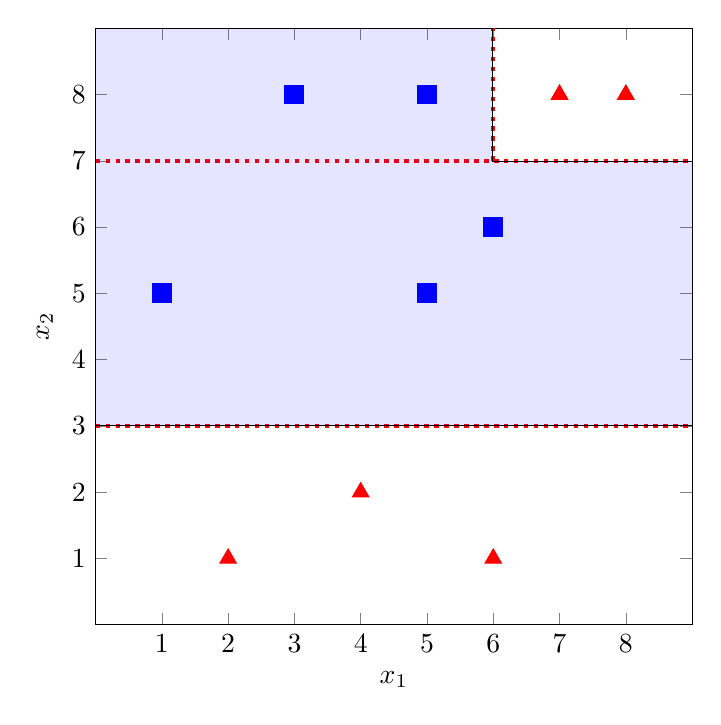
\begin{tikzpicture}
            \begin{axis}[
                scale=0.9, width=10cm, height=10cm, mark options={scale=1.7},
                xmin=0, xmax=9, xtick={1,2,3,4,5,6,7,8},
                ymin=0, ymax=9, ytick={1,2,3,4,5,6,7,8},
                samples=50, xlabel=$x_1$, ylabel=$x_2$]]
                \addplot[red, ultra thick, dotted] coordinates { (0,3) (9,3) };
                \addplot[red, ultra thick, dotted] coordinates { (0,7) (9,7) };
                \addplot[red, ultra thick, dotted] coordinates { (6,7) (6,9) };
                \addplot[fill=blue, fill opacity=0.1] coordinates { (0, 3.01) (9, 3.01) (9, 6.99) (5.99, 6.99) (5.99, 9) (0, 9) (0, 3.01) } \closedcycle;
                \addplot [
                    scatter,
                    only marks,
                    point meta=explicit symbolic,
                    scatter/classes={
                        a={mark=triangle*,red},
                        b={mark=square*,blue}
                    },
                    nodes near coords*={},
                    visualization depends on={\thisrow{myvalue} \as \myvalue},
                ] table [meta=label] {
                    x y label myvalue
                    2 1 a 1
                    4 2 a 1
                    6 1 a 1
                    1 5 b 1
                    5 5 b 1
                    6 6 b 1
                    3 8 b 1
                    5 8 b 1
                    7 8 a 1
                    8 8 a 1
                };
            \end{axis}
            \end{tikzpicture} 
        \end{center}
    \end{soln}
    \begin{qauthor}
        Henry
    \end{qauthor}
    
    \part[3] \textbf{Fill in the blank:} Complete the following paragraph about training decision trees by circling the best of the provided options for each of blanks: 
    
    \doublespacing
    \begin{quote}
            Paloma the Possum is training a decision tree and notices that there is a \underline{\quad large \quad / \quad small \quad} difference between her training and test error rates, a classic sign of overfitting. 
            
            She suspects this is because the maximum depth that she allowed her decision tree to grow to, a model \underline{\quad parameter \quad / \quad hyperparameter \quad}, was too \underline{\quad large \quad / \quad small \quad}.
    \end{quote}
    \singlespacing
    
    \begin{soln}
        Paloma the Possum is training a decision tree and notices that there is a large difference between her training and test error rates, a classic sign of overfitting. She suspects this is because the maximum depth that she allowed her decision tree to grow to, a model hyperparameter, was too large.
    \end{soln}
    \begin{qauthor}
        Bhargav, Judge whether a decision tree is "underfitting" or "overfitting", Plan an experiment that uses training, validation, and test datasets to predict the performance of a classifier on unseen data (without cheating)

        Edited by Henry
    \end{qauthor}
    
\end{parts}
